%! Author = joels
%! Date = 27/01/2022

\section{Einführung}
\textbf{Wieso Compilerbau?}
\begin{itemize}[topsep=0pt]
    \itemsep -0.4em
    \item Sprachkonzepte verstehen
    \item Einschränkungen und Kosten von Sprachfeatures beurteilen können
    \item Konzepte in verwandten Bereichen einsetzen: Converter, Analysen, Entwicklertools, Algorithmen
\end{itemize}
\textbf{Compiler:} Transformiert Quellcode einer Programmiersprache in ausführbaren Maschinencode.\\
\textbf{Runtime System:} Unterstützt die Ausführung mit software- und Hardware-Mechanismen

\subsection{Architekturen}
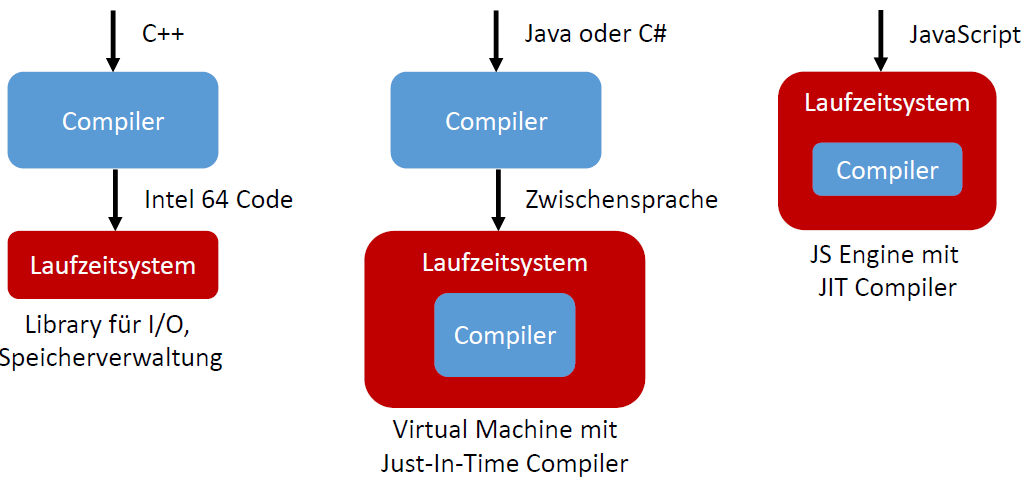
\includegraphics[width=0.7\linewidth]{architekturen}

\subsection{Aufbau Compiler}
\begin{minipage}{0,3\linewidth}
    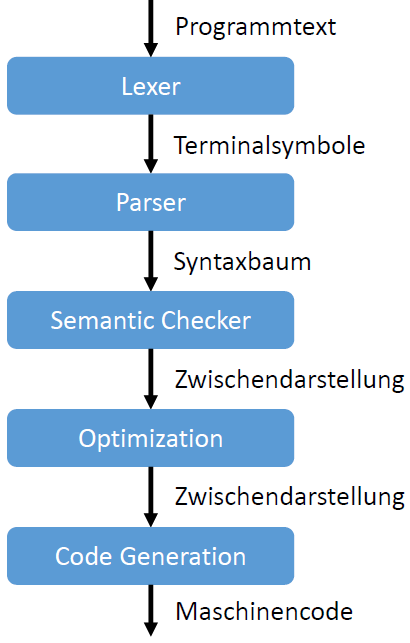
\includegraphics[width=\linewidth]{aufbau_compiler}
\end{minipage}
\begin{minipage}{0,7\linewidth}
    \begin{itemize}[topsep=0pt]
        \itemsep -0.2em
        \item Lexer (Lexikanische Analyse, Scanner)
        \SubItem{Zerlegt Programmtext in Terminalsymbole (Tokens)}
        \item Parser (Syntaktische Analyse)
        \SubItem{Erzeugt Syntaxbaum gemäss Programmstruktur}
        \item Semantic Checker (Schemantische Analyse)
        \SubItem{Löst Symbole auf, prüft Typen und semantische regeln}
        \item Optimization (Optional)
        \SubItem{Wandelt Zwischendarstellung in effizientere um}
        \item Code Generation
        \SubItem{Erzeugt ausführbaren maschinencode}
        \item Zwischendarstellung (Intermediate Representation)
        \SubItem{Beschreibt Programm als Datenstruktur (diverse varianten)}
    \end{itemize}
\end{minipage}

\subsection{Aufbau Laufzeitsystem}
\begin{minipage}{0,3\linewidth}
    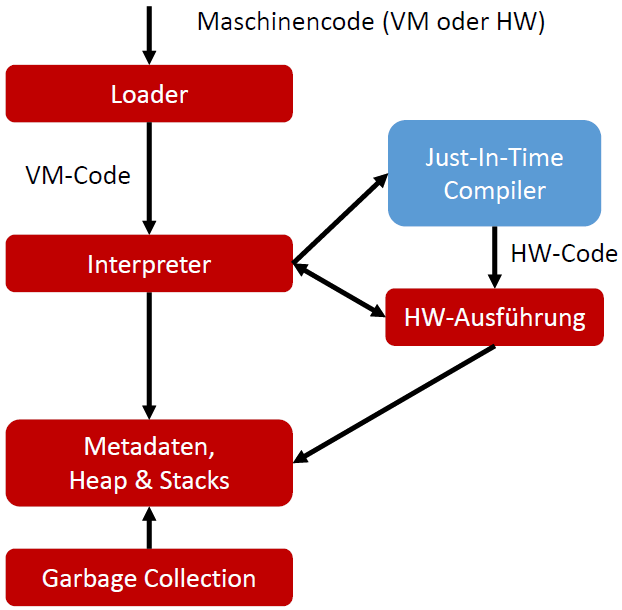
\includegraphics[width=\linewidth]{aufbau_laufzeitsystem}
\end{minipage}
\begin{minipage}{0,7\linewidth}
    \begin{itemize}[topsep=0pt]
        \itemsep -0.2em
        \item Loader
        \SubItem{Lädt maschinencode in Speicher, veranlasst Ausführung}
        \item Interpreter
        \SubItem{Liest Instruktionen und emuliert diese in Software}
        \item JIT Compiler
        \SubItem{Übersetzt Code-Teile in hardware-Instruktionscode}
        \item HW-Ausführung (nativ)
        \SubItem{Lässt Instruktionscode direkt auf HW-Prozessor laufen}
        \item Metadaten, heap + Stacks
        \SubItem{Merken programminfos, Objekte und Prozeduralaufrufe}
        \item Garbage Collection
        \SubItem{Räumt nicht erreichbare Objekte ab}
    \end{itemize}
\end{minipage}

\subsection{EBNF (Extended Backus Naur Form)}
\textbf{Definition einer Programmiersprache:} Syntax (mittels Regeln/Formeln), Semantik (meist in Prosa)
\subsubsection{EBNF Konstrukte}
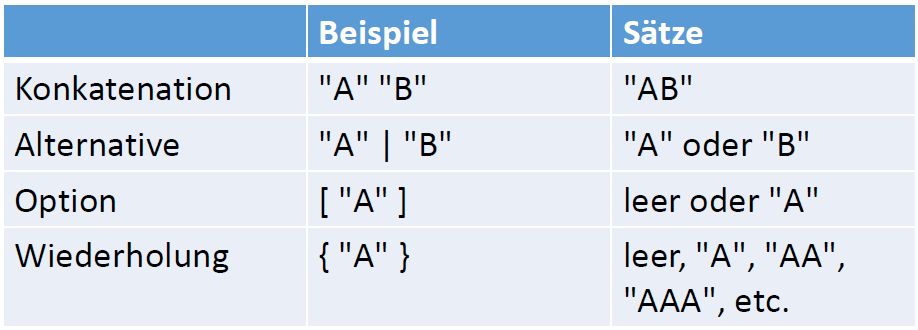
\includegraphics[width=0.7\linewidth]{ebnf_konstrukte}

\subsubsection{Arithmetische Adrücke}
\begin{minipage}{0,6\linewidth}
    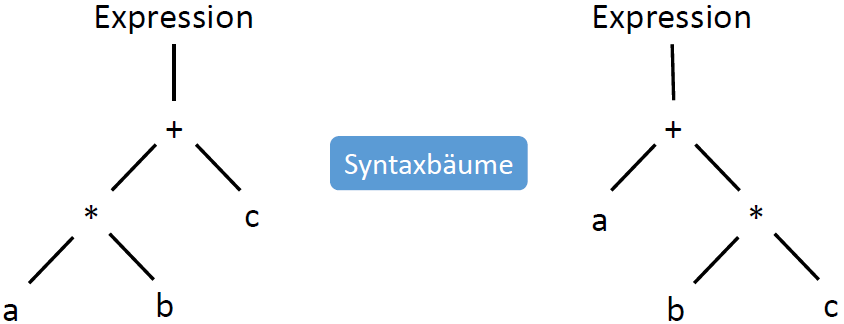
\includegraphics[width=\linewidth]{ebnf_ausdruecke}
\end{minipage}
\begin{minipage}{0,4\linewidth}
    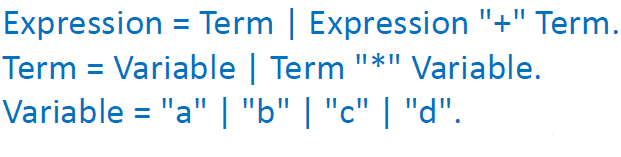
\includegraphics[width=\linewidth]{ebnf_ausdruecke_loesung}
\end{minipage}
\subsubsection{Explizite Klammerungen}
\begin{minipage}{0,4\linewidth}
    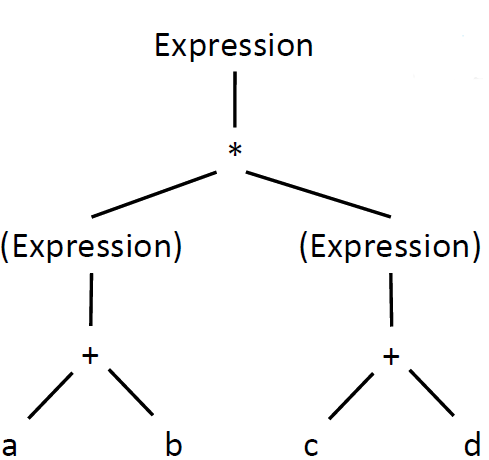
\includegraphics[width=\linewidth]{ebnf_ausdruecke_klammern}
\end{minipage}
\begin{minipage}{0,6\linewidth}
    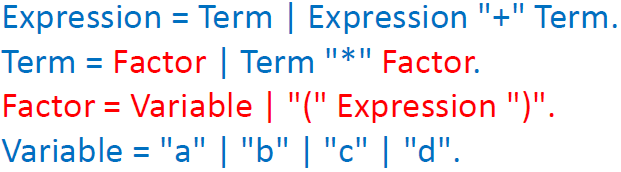
\includegraphics[width=\linewidth]{ebnf_ausdruecke_klammern_loesung}
    \\
    \linebreak
    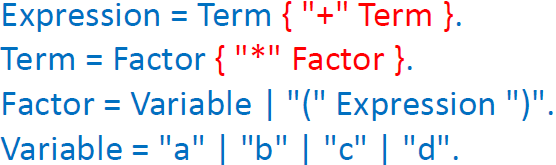
\includegraphics[width=\linewidth]{ebnf_ausdruecke_klammern_loesung_2}
\end{minipage}